При большом количестве объектов на изображении происходит ощутимая просадка частоты работы при использовании алгоритмов с ReID моделями. 
Это связано с тем, что их вычисления невозможно перенести на TPU в связи с произвольным размером входа.  
Четвертым экспериментом было решено провести исследование величин этих просадок. 

По результатам эксперимента получена таблица получена таблица \ref{tab:correlation_fps_objectcount}. 
\begin{table}[htbp]
\caption{Корреляция частоты работы с количеством объектов на изображении}
\label{tab:correlation_fps_object}
\centering
\begin{tabular}{lr}
\toprule
Алгоритм & Корреляция \\
\midrule
BoT-SORT & -0.63 \\
ByteTrack & -0.03 \\
Deep OC-SORT & -0.65 \\
ImprAssOC & -0.63 \\
OC-SORT & -0.10 \\
StrongSORT & -0.66 \\
\bottomrule
\end{tabular}

\end{table}

\begin{figure}[ht]
    \centering
    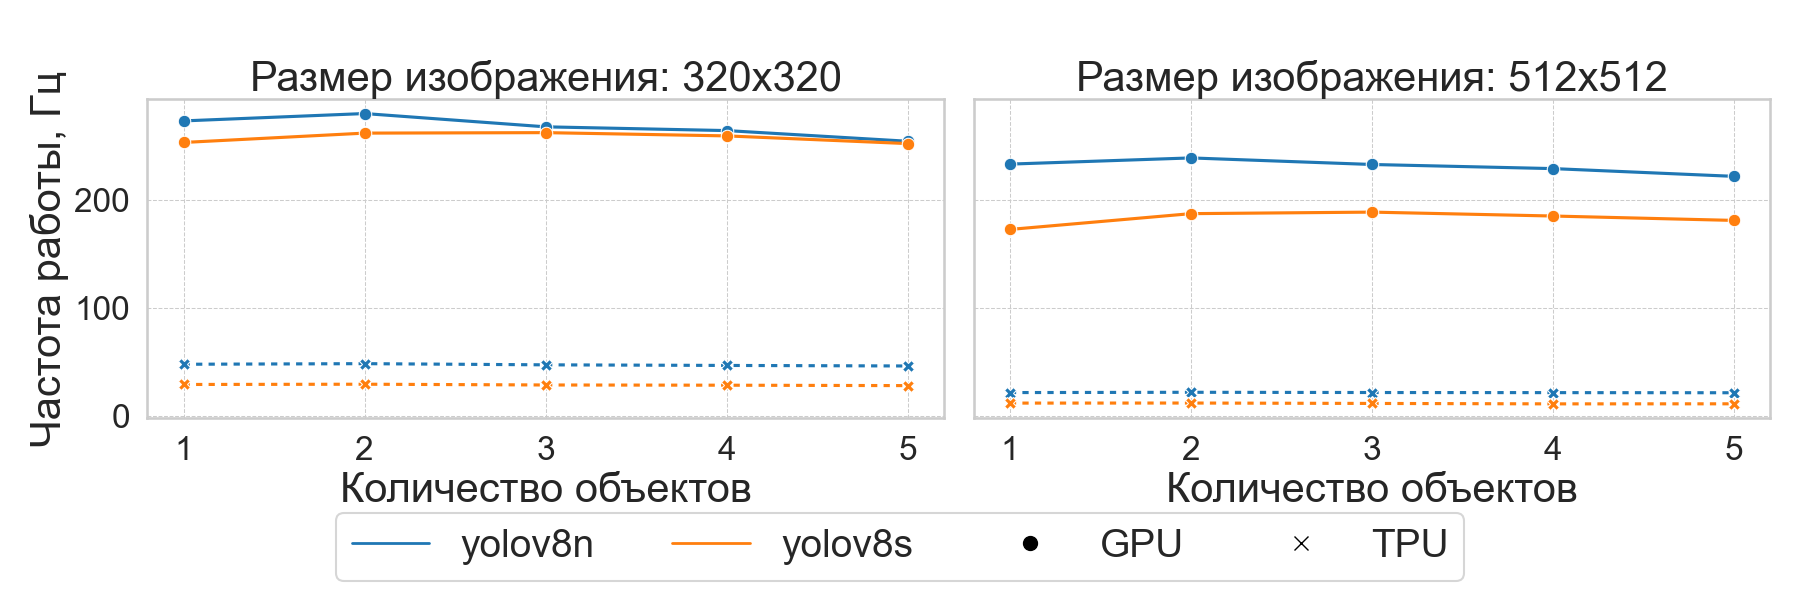
\includegraphics[width=1\textwidth]{plots/fps_vs_object_count/ByteTrack_gpu_tpu.png}
    \caption{График зависимости частоты работы алгоритма ByteTrack от количества объектов на изображении}
    \label{fig:fps_object_ByteTrack}
\end{figure}

\begin{figure}[ht]
    \centering
    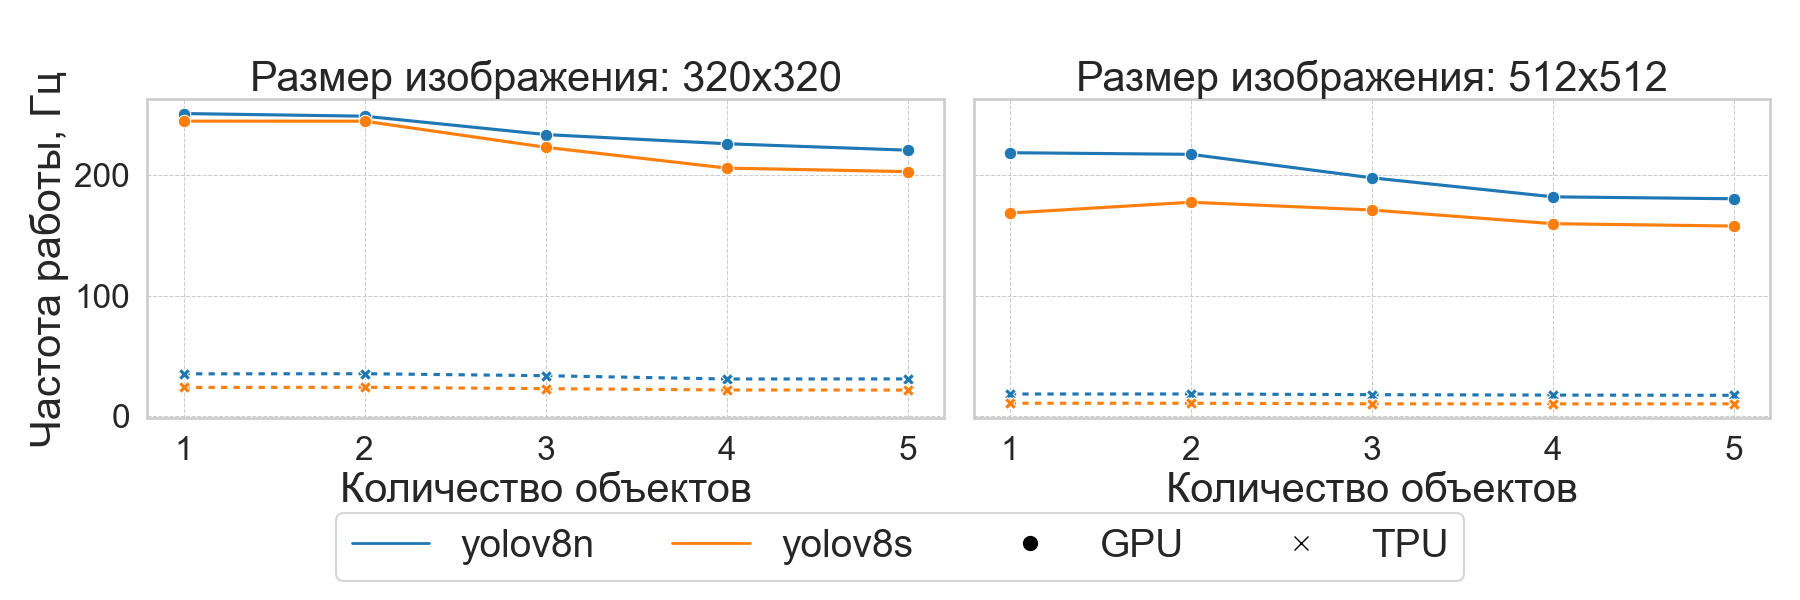
\includegraphics[width=1\textwidth]{plots/fps_vs_object_count/OC-SORT_gpu_tpu.png}
    \caption{График зависимости частоты работы алгоритма OC-SORT от количества объектов на изображении}
    \label{fig:fps_object_OC-SORT}
\end{figure}

\begin{figure}[ht]
    \centering
    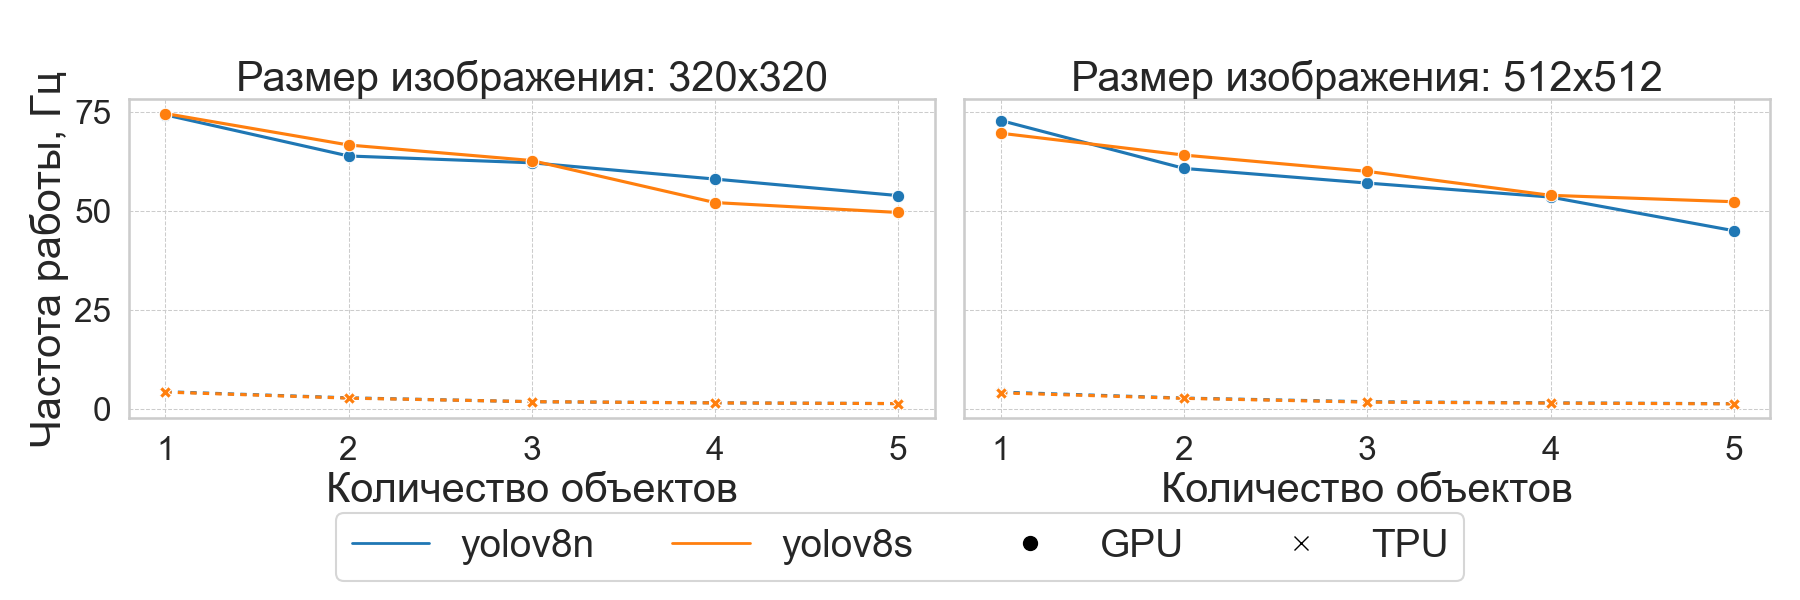
\includegraphics[width=1\textwidth]{plots/fps_vs_object_count/Deep OC-SORT_gpu_tpu.png}
    \caption{График зависимости частоты работы алгоритма Deep OC-SORT от количества объектов на изображении}
    \label{fig:fps_object_Deep OC-SORT}
\end{figure}

\begin{figure}[ht]
    \centering
    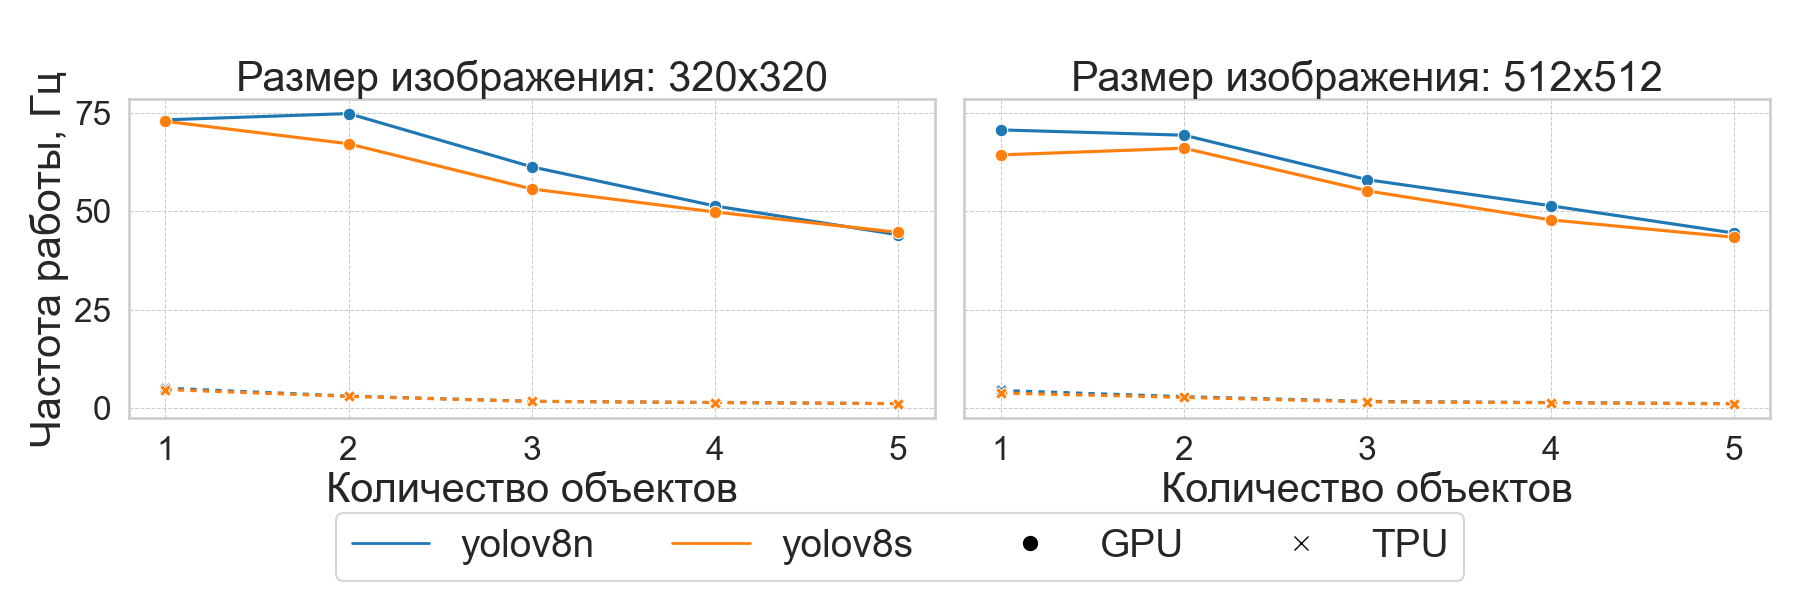
\includegraphics[width=1\textwidth]{plots/fps_vs_object_count/StrongSORT_gpu_tpu.png}
    \caption{График зависимости частоты работы алгоритма StrongSORT от количества объектов на изображении}
    \label{fig:fps_object_StrongSORT}
\end{figure}

\begin{figure}[ht]
    \centering
    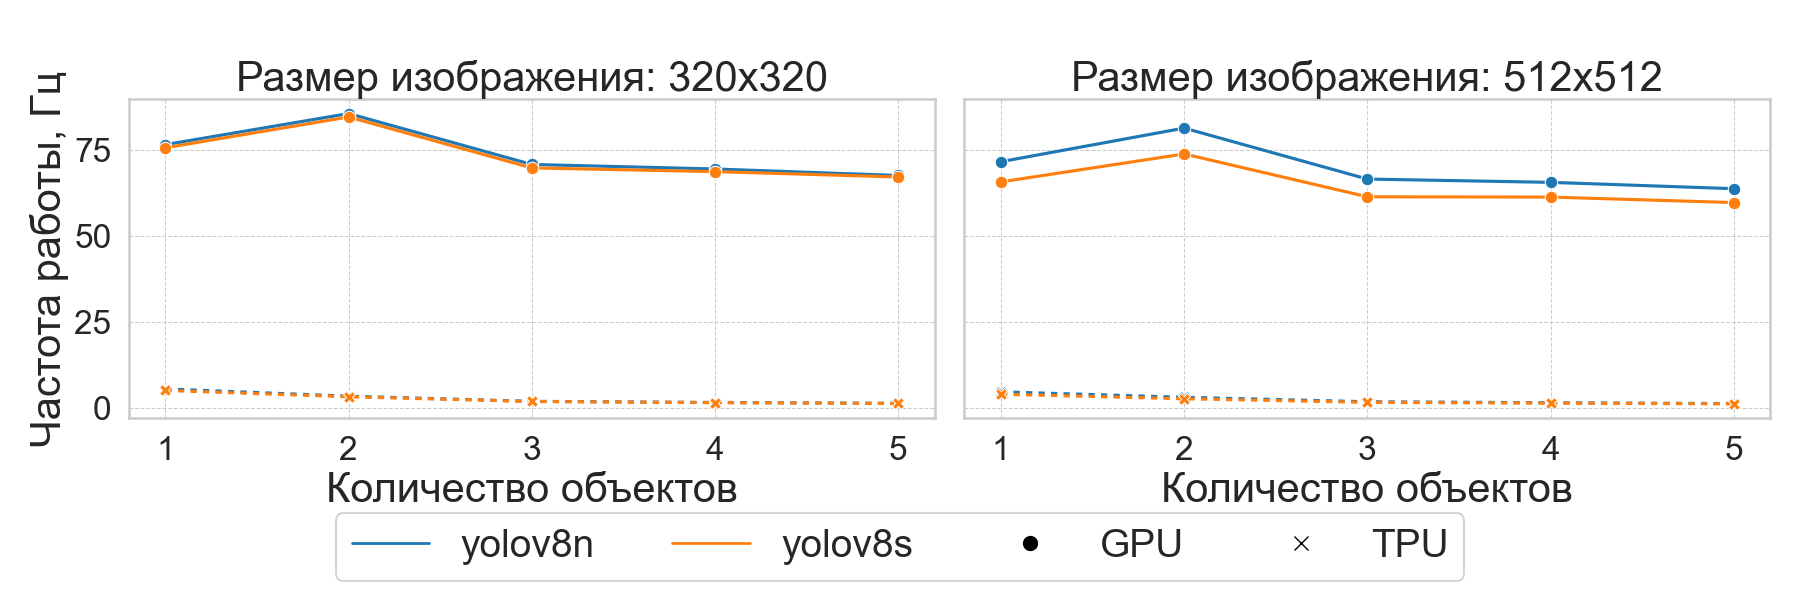
\includegraphics[width=1\textwidth]{plots/fps_vs_object_count/BoT-SORT_gpu_tpu.png}
    \caption{График зависимости частоты работы алгоритма BoT-SORT от количества объектов на изображении}
    \label{fig:fps_object_BoT-SORT}
\end{figure}

\begin{figure}[ht]
    \centering
    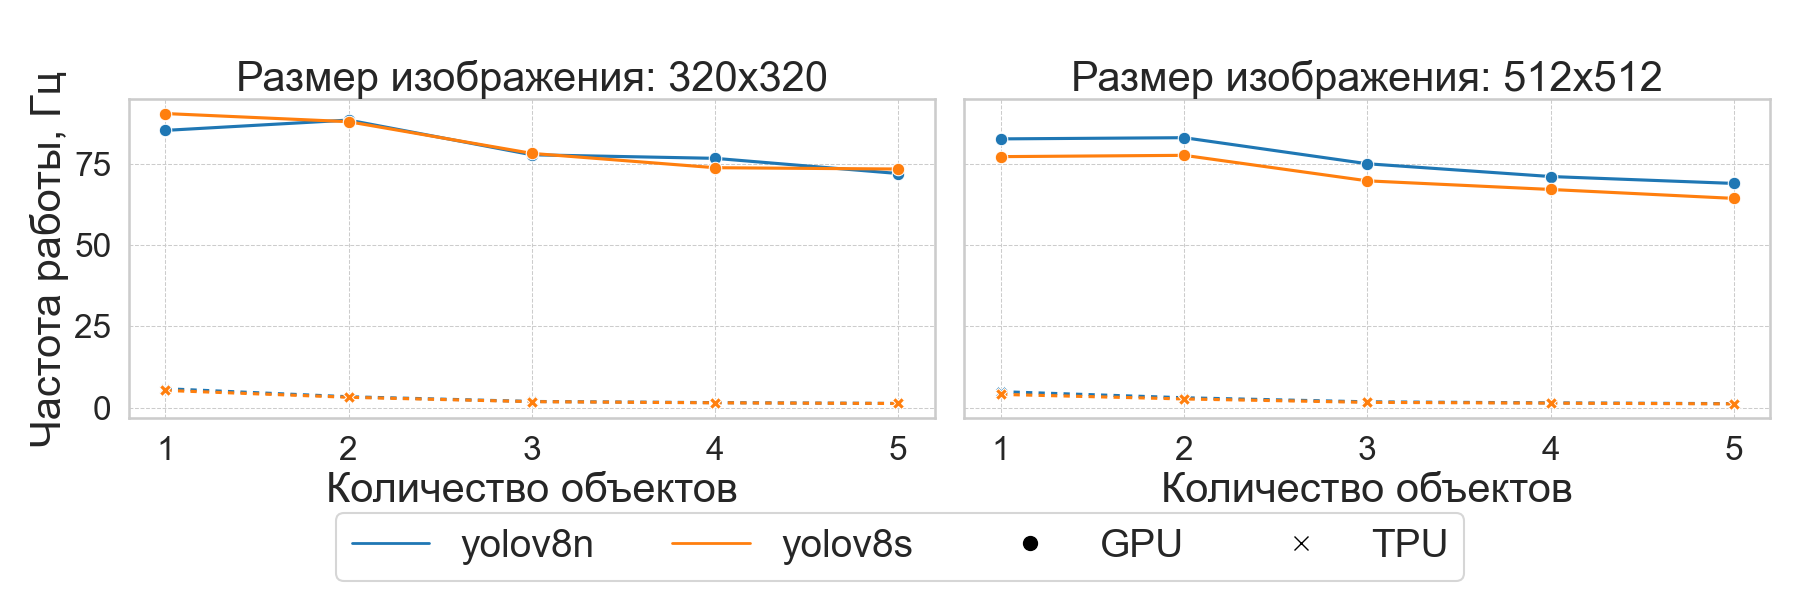
\includegraphics[width=1\textwidth]{plots/fps_vs_object_count/ImprAssOC_gpu_tpu.png}
    \caption{График зависимости частоты работы алгоритма ImprAssOC от количества объектов на изображении}
    \label{fig:fps_object_ImprAssOC}
\end{figure}
\FloatBarrier